\documentclass[12pt, a4paper]{article}
\usepackage{graphicx}
\usepackage{xurl}
\usepackage{geometry}
\usepackage{float}
\usepackage{indentfirst}
\geometry{left=2.54cm, right=2.54cm, top=3.18cm, bottom=3.18cm}
% \setlength{\parindent}{0pt}

\title{Weekly Report}
\author{Jerry Jin}

\begin{document}

\maketitle

\section*{Week 12/11}

\subsection*{Goals}

\begin{itemize}
    \item Transfer of learning from gains to synapses in Swinehart and Abbott (2005).

    \item Transfer of learning from gains to synapses in RNN.

\end{itemize}

\newpage

\subsection*{Transfer of learning in Simple Feedforward Network}

I realize the transfer of learning in the Simple Feedforward Network from Swinehart and Abbott (2005).

In the first 200 epochs of training, I use only SGD on gains and shifts to let the network quickly reduce its loss. Then, I start the Oja learning. But Oja learning only happens when the current loss is small enough.  Then, after another 100 epochs, I start the shrinkage of gains and shifts towards its initial value, where $g_i=3$ and $s_i=1$. The shrinkage is realized by imposing boundaries, both passively and actively. For example, if $g_i=5$ currently, the passive boundary for $g_i$ would be $[3,5]$, and an active shrinkage might happen to let the boundary become $[3,3+\gamma(5-3)]$. For now, the $\gamma=0.0001$.

I find that Oja's learning more stable than normal Hebbian learning. What's more, the performance of the network depends heavily on choosing a good Oja's $\alpha$. In Oja's learning, $w_{ij} \rightarrow w_{ij} + \eta (r_i r_j - \alpha r_j^2 w_{ij})$, $||w||^2$ would converge to $1/\alpha$. To make the whole procedure work, there should exist a weight solution with $||w||^2=1/\alpha$ using initial gains and shifts. For now, $\alpha=12$.

\begin{figure}[H]
    \centering
    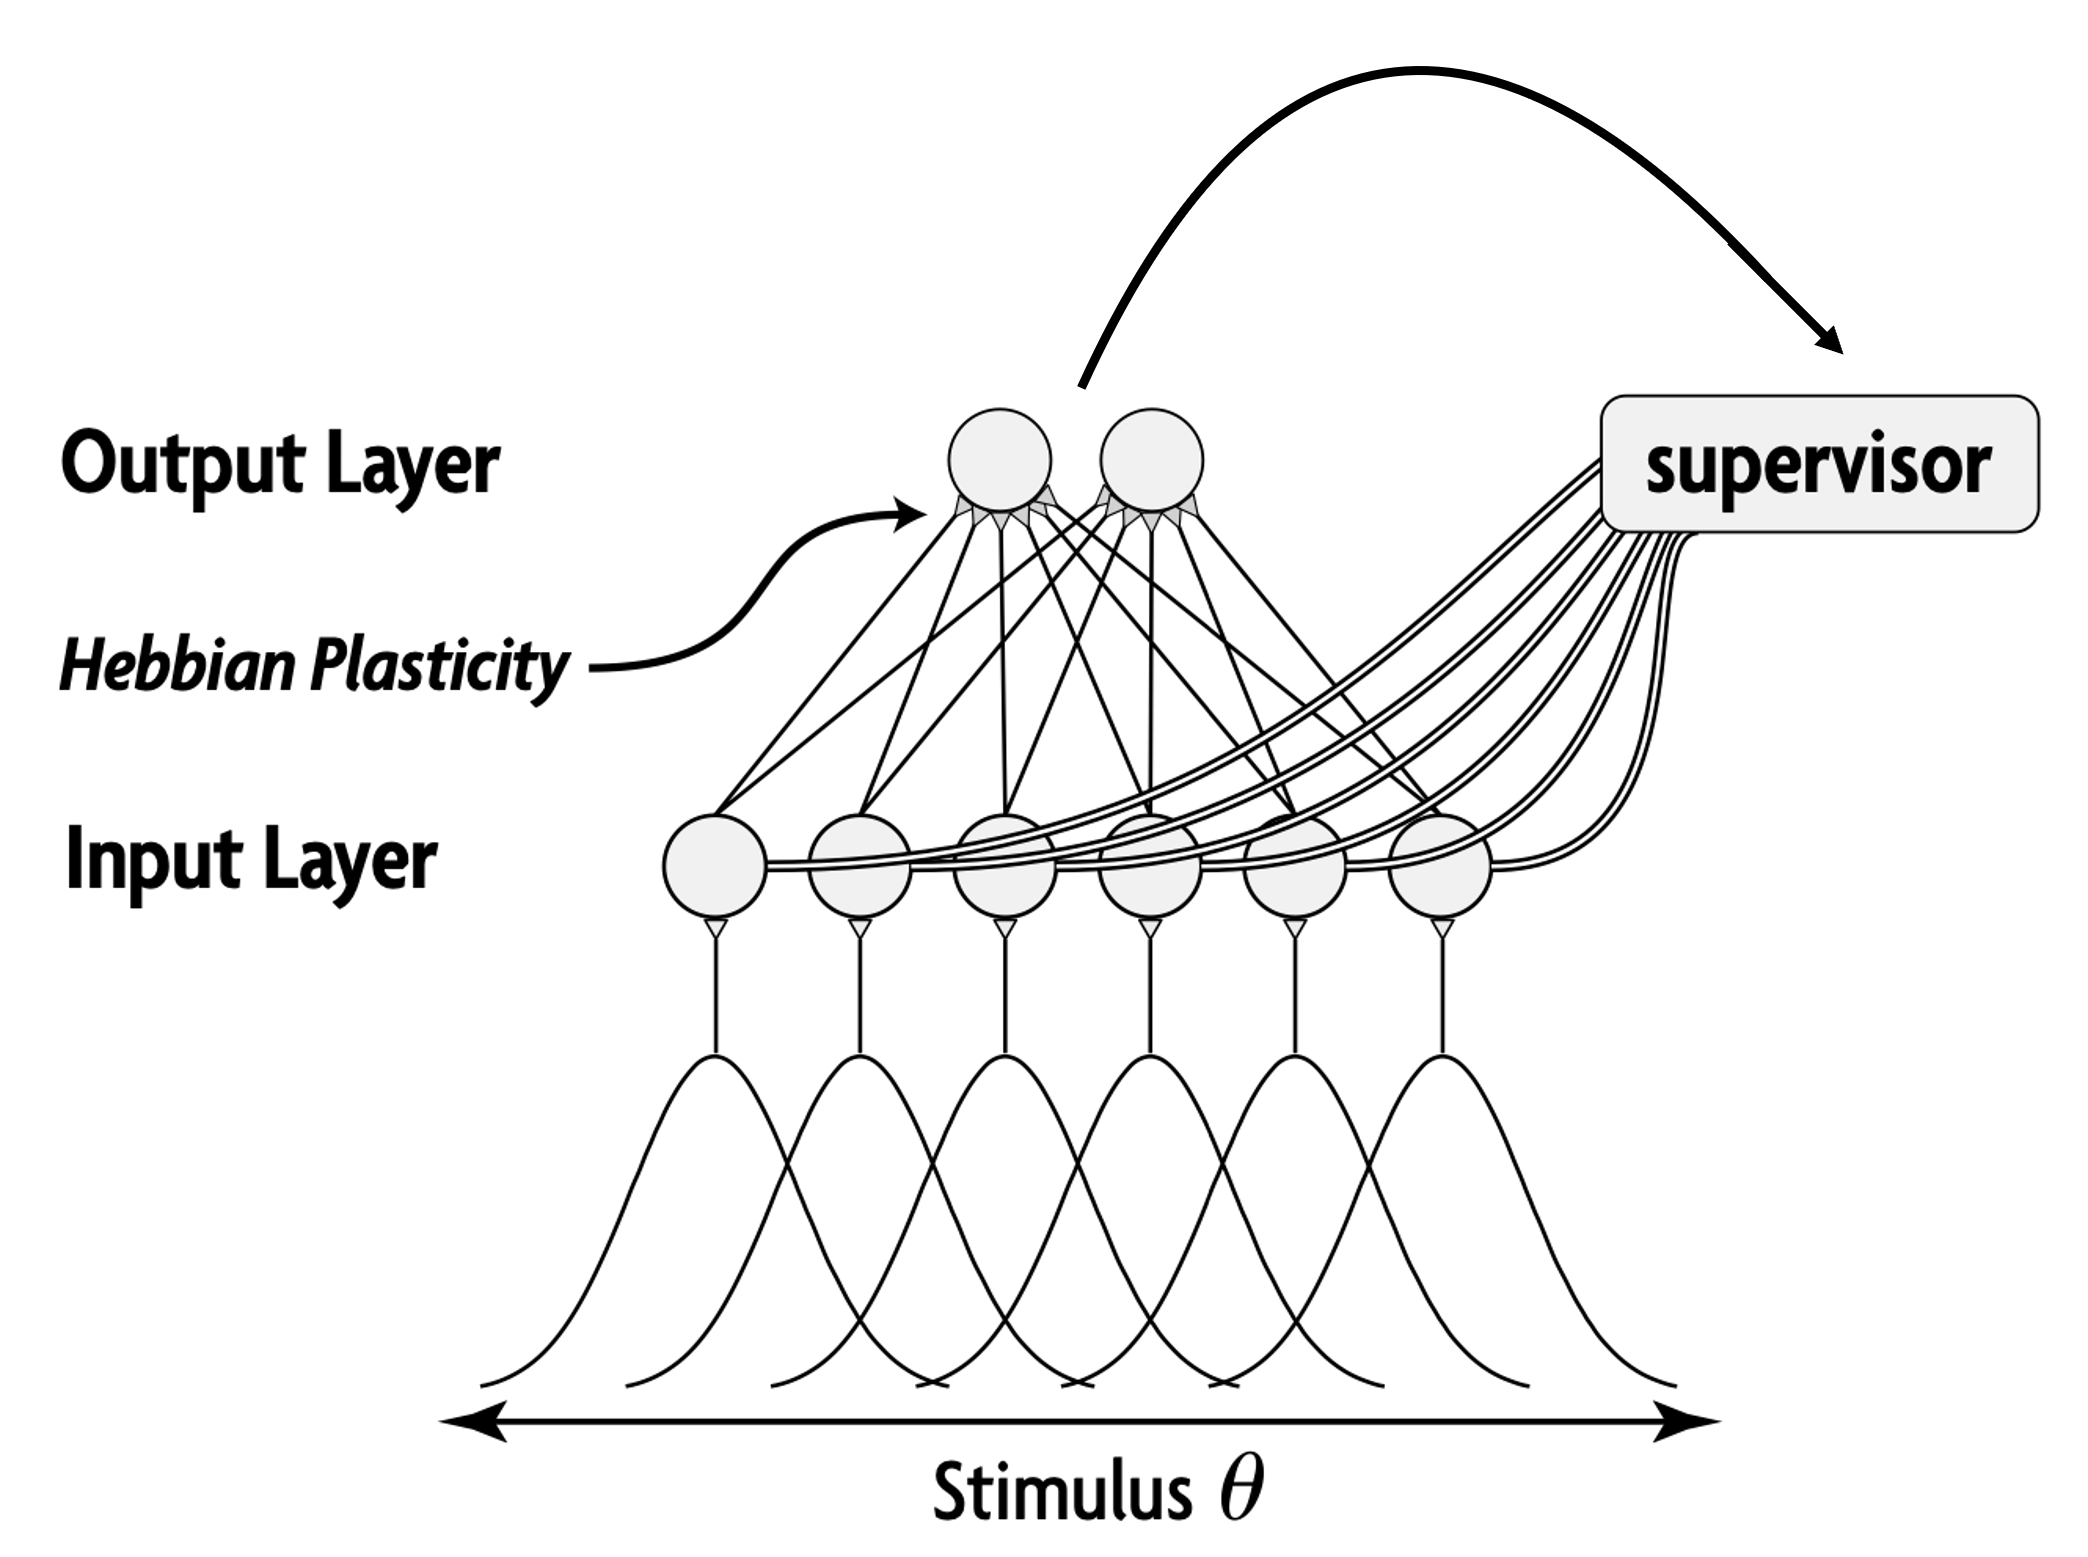
\includegraphics[width=0.6\textwidth]{fig/abb05_struc.png}
    \label{fig:1}
\end{figure}

\begin{figure}[H]
    \centering
    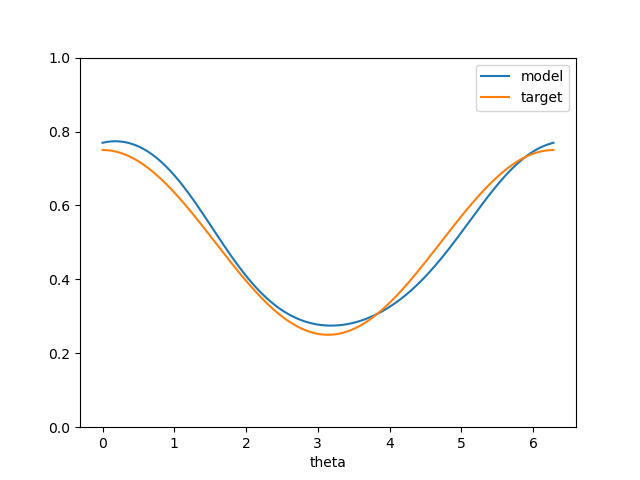
\includegraphics[width=0.6\textwidth]{fig/abb05_outputs_nosup.png} \\
    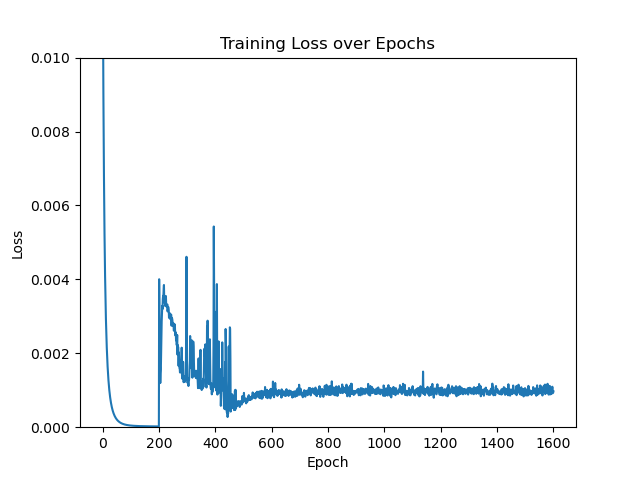
\includegraphics[width=0.45\textwidth]{fig/abb05_loss.png}
    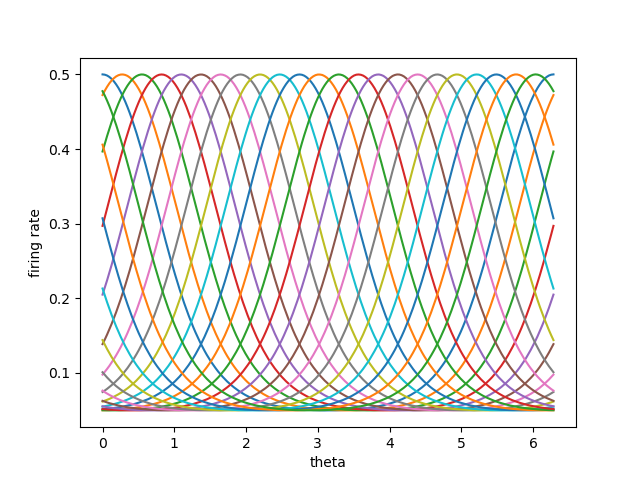
\includegraphics[width=0.45\textwidth]{fig/abb05_rf.png}
    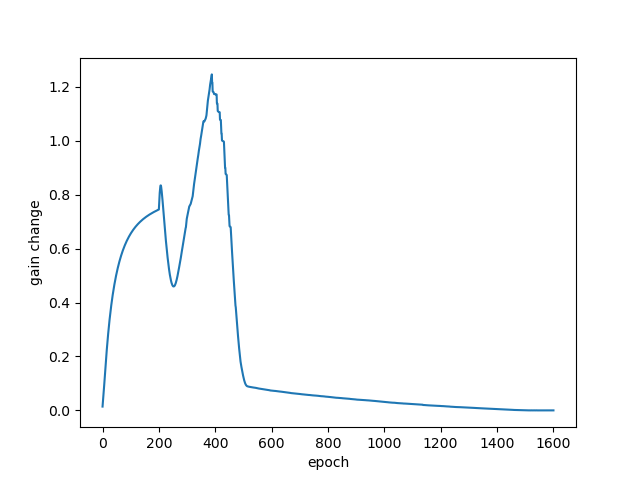
\includegraphics[width=0.45\textwidth]{fig/abb05_gc.png}
    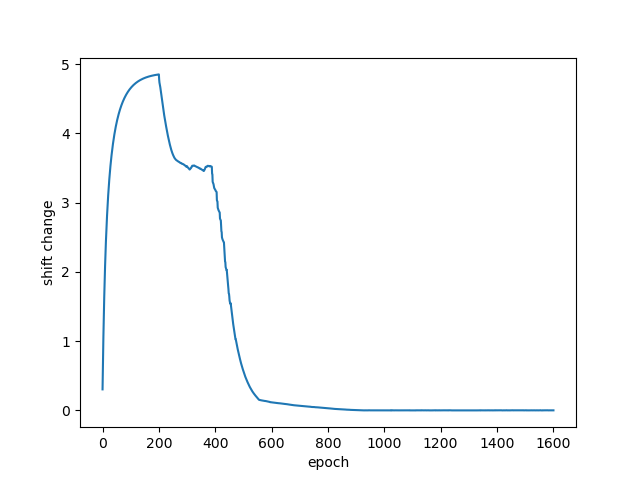
\includegraphics[width=0.45\textwidth]{fig/abb05_sc.png}
    \label{fig:1}
\end{figure}

\newpage

\subsection*{Transfer of learning in RNN}

I try to implement a similar procedure in training my RNN. But it is not performing well so far. Parameters need to be tuned.

The loss is converging at a certain value. This might be because the choice of Oja's $\alpha$ is not optimal. Also, hebbian learning for inhibitory synapses might also be necessary to reach a good balanced state. What's more, different from the Simple Feedforward Network, the input matrix and output matrix now in RNN is a random matrix. Maybe a carefully-designed matrix would be helpful.

\begin{figure}[H]
    \centering
    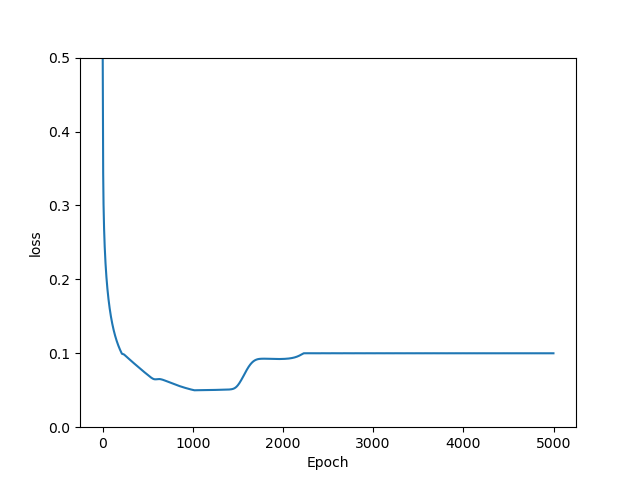
\includegraphics[width=0.45\textwidth]{fig/sin_gn_loss.png} \\
    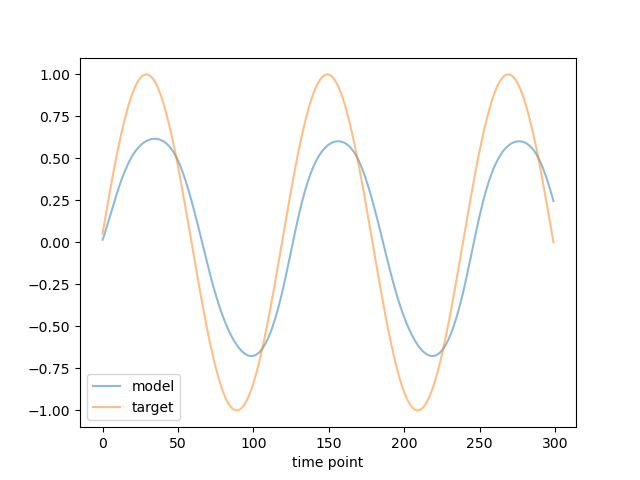
\includegraphics[width=0.45\textwidth]{fig/sin_gn_train.png}
    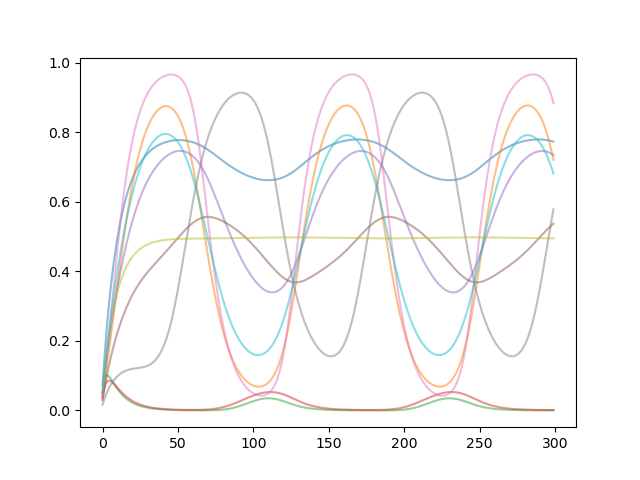
\includegraphics[width=0.45\textwidth]{fig/sin_gn_ind.png}
    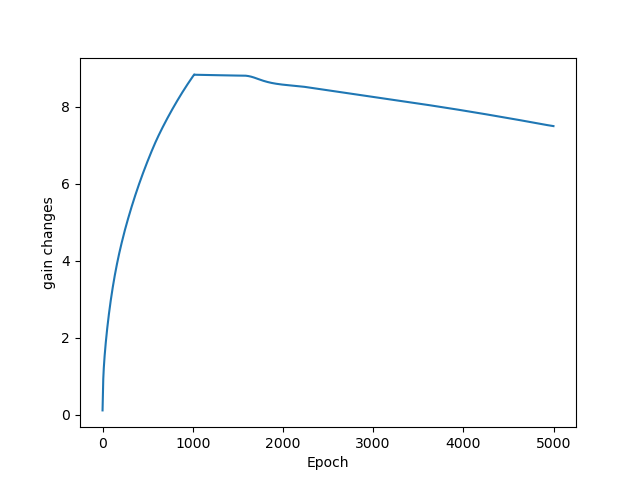
\includegraphics[width=0.45\textwidth]{fig/sin_gn_gc.png}
    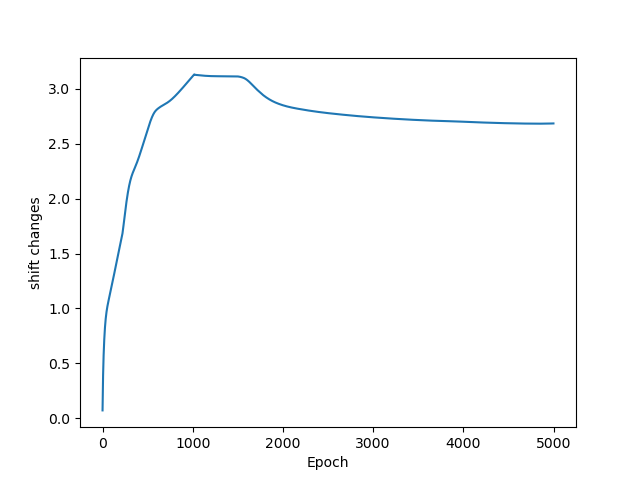
\includegraphics[width=0.45\textwidth]{fig/sin_gn_sc.png}
    \label{fig:1}
\end{figure}

\newpage

\end{document}